% Standalone Helix: 4 Nov 2026 Research Meeting
% Visual style follows the 21 Oct 2026 light Madrid decks.
% Facts are taken from the local ASPLOS '25 PDF only.
% Compile with pdfLaTeX from this directory. Keep Helix/ beside this file.
\documentclass[aspectratio=169,10pt]{beamer}
\usepackage[english]{babel}
\usepackage[utf8]{inputenc}
\usepackage[T1]{fontenc}
\usepackage{lmodern}
\usepackage{amsmath,amssymb}
\usepackage{booktabs,tabularx,array}
\usepackage{graphicx}
\graphicspath{{./}{figures/}}
\usepackage{xcolor}
\usepackage{tikz}
\usetikzlibrary{arrows.meta,positioning,calc,shapes.geometric}
\usepackage{hyperref}

\usetheme{Madrid}
\usecolortheme{default}
\definecolor{Ink}{HTML}{243748}
\definecolor{Muted}{HTML}{667B8B}
\definecolor{Accent}{HTML}{347E74}
\definecolor{AccentBlue}{HTML}{507DAD}
\definecolor{SoftMint}{HTML}{E6F4EE}
\definecolor{SoftBlue}{HTML}{E9F2F9}
\definecolor{SoftLilac}{HTML}{F1EEF8}
\definecolor{Paper}{HTML}{FBFCFE}
\definecolor{Divider}{HTML}{D8E4EB}

\setbeamercolor{background canvas}{bg=Paper}
\setbeamercolor{normal text}{fg=Ink}
\setbeamercolor{structure}{fg=Accent}
\setbeamercolor{frametitle}{fg=Ink,bg=SoftBlue}
\setbeamercolor{title}{fg=Ink}
\setbeamercolor{subtitle}{fg=Muted}
\setbeamercolor{block title}{fg=Ink,bg=SoftBlue}
\setbeamercolor{block body}{fg=Ink,bg=white}
\setbeamercolor{item}{fg=Accent}
\setbeamercolor{caption name}{fg=Muted}
\setbeamercolor{footline}{fg=Muted,bg=Paper}
\setbeamerfont{frametitle}{size=\large,series=\bfseries}
\setbeamerfont{footline}{size=\tiny}
\setbeamerfont{block title}{series=\bfseries}
\setbeamertemplate{headline}{}
\setbeamertemplate{navigation symbols}{}
\setbeamertemplate{blocks}[rounded][shadow=false]
\setbeamertemplate{itemize items}[circle]
\setbeamertemplate{enumerate items}[default]
\setbeamertemplate{itemize subitem}[circle]
\setbeamertemplate{footline}{%
  \leavevmode\hbox{%
    \begin{beamercolorbox}[wd=\paperwidth,ht=.30cm,dp=.16cm,rightskip=.60cm plus 1fil]{footline}%
      \hspace{.45cm}\insertsectionhead\hfill\hyperlink{INDEX}{Discussion index}\hspace{.45cm}\insertframenumber\,/\,\inserttotalframenumber
    \end{beamercolorbox}}}
\setbeamertemplate{frametitle}{%
  \nointerlineskip
  \begin{beamercolorbox}[wd=\paperwidth,ht=.72cm,dp=.16cm,leftskip=.55cm,rightskip=.40cm]{frametitle}%
    \usebeamerfont{frametitle}\insertframetitle
  \end{beamercolorbox}}

\newcommand{\smalllabel}[1]{{\scriptsize\bfseries\color{Accent}\MakeUppercase{#1}}}
\newcommand{\hint}[1]{{\scriptsize\color{Muted}#1}}
\newcommand{\stepcard}[3]{%
  \begin{beamercolorbox}[rounded=true,sep=0.10cm,wd=\linewidth]{block body}%
    {\scriptsize\bfseries\color{Accent}#1}\par\vspace{.4mm}
    {\footnotesize\bfseries #2}\par\vspace{.4mm}
    {\scriptsize\color{Muted}#3}%
  \end{beamercolorbox}}

% Missing assets are build errors, never silent placeholders.
\newcommand{\figureplaceholder}[3]{\par{\centering\includegraphics[width=\linewidth,height=#2,keepaspectratio]{#1}\par}}
\setbeamersize{text margin left=.45cm,text margin right=.45cm}
\newcommand{\nav}[2]{\hyperlink{#1}{\beamerbutton{#2}}}
\newcommand{\slidenote}[2]{\par\vfill{\scriptsize\color{Muted}Source: Helix, #1}\hfill #2\par}
\newcommand{\back}[2][]{\par\vspace{.12cm}\nav{#2}{Main \ref*{#2}}\ #1\hfill\nav{INDEX}{Discussion Index}}
\newcommand{\meta}[1]{{\small\color{Muted}#1}\par\medskip}
\newcommand{\point}[2]{\par\textbf{\color{Accent}#1}\quad #2\par\medskip}
\newcommand{\src}[1]{\par\vfill\hint{Source: Helix, #1}}

\title[Helix]{Helix: Serving LLMs over Heterogeneous GPUs and Network via Max-Flow}
\subtitle{Joint Model Placement and Per-Request Scheduling}
\author{Yu-Jui Liang}
\institute{National Taiwan University \quad | \quad Academia Sinica}
\date{4 Nov 2026}
\subject{Research meeting, 4 Nov 2026}

% Two viewports of the supplied caption-free Fig. 2, never resampled.
% PNG has no DPI metadata: pdfTeX interprets one pixel as one bp.
% Preserve both diagrams, weights table, payload sizes and every capacity.
\newcommand{\flowpanels}{%
 {\centering
 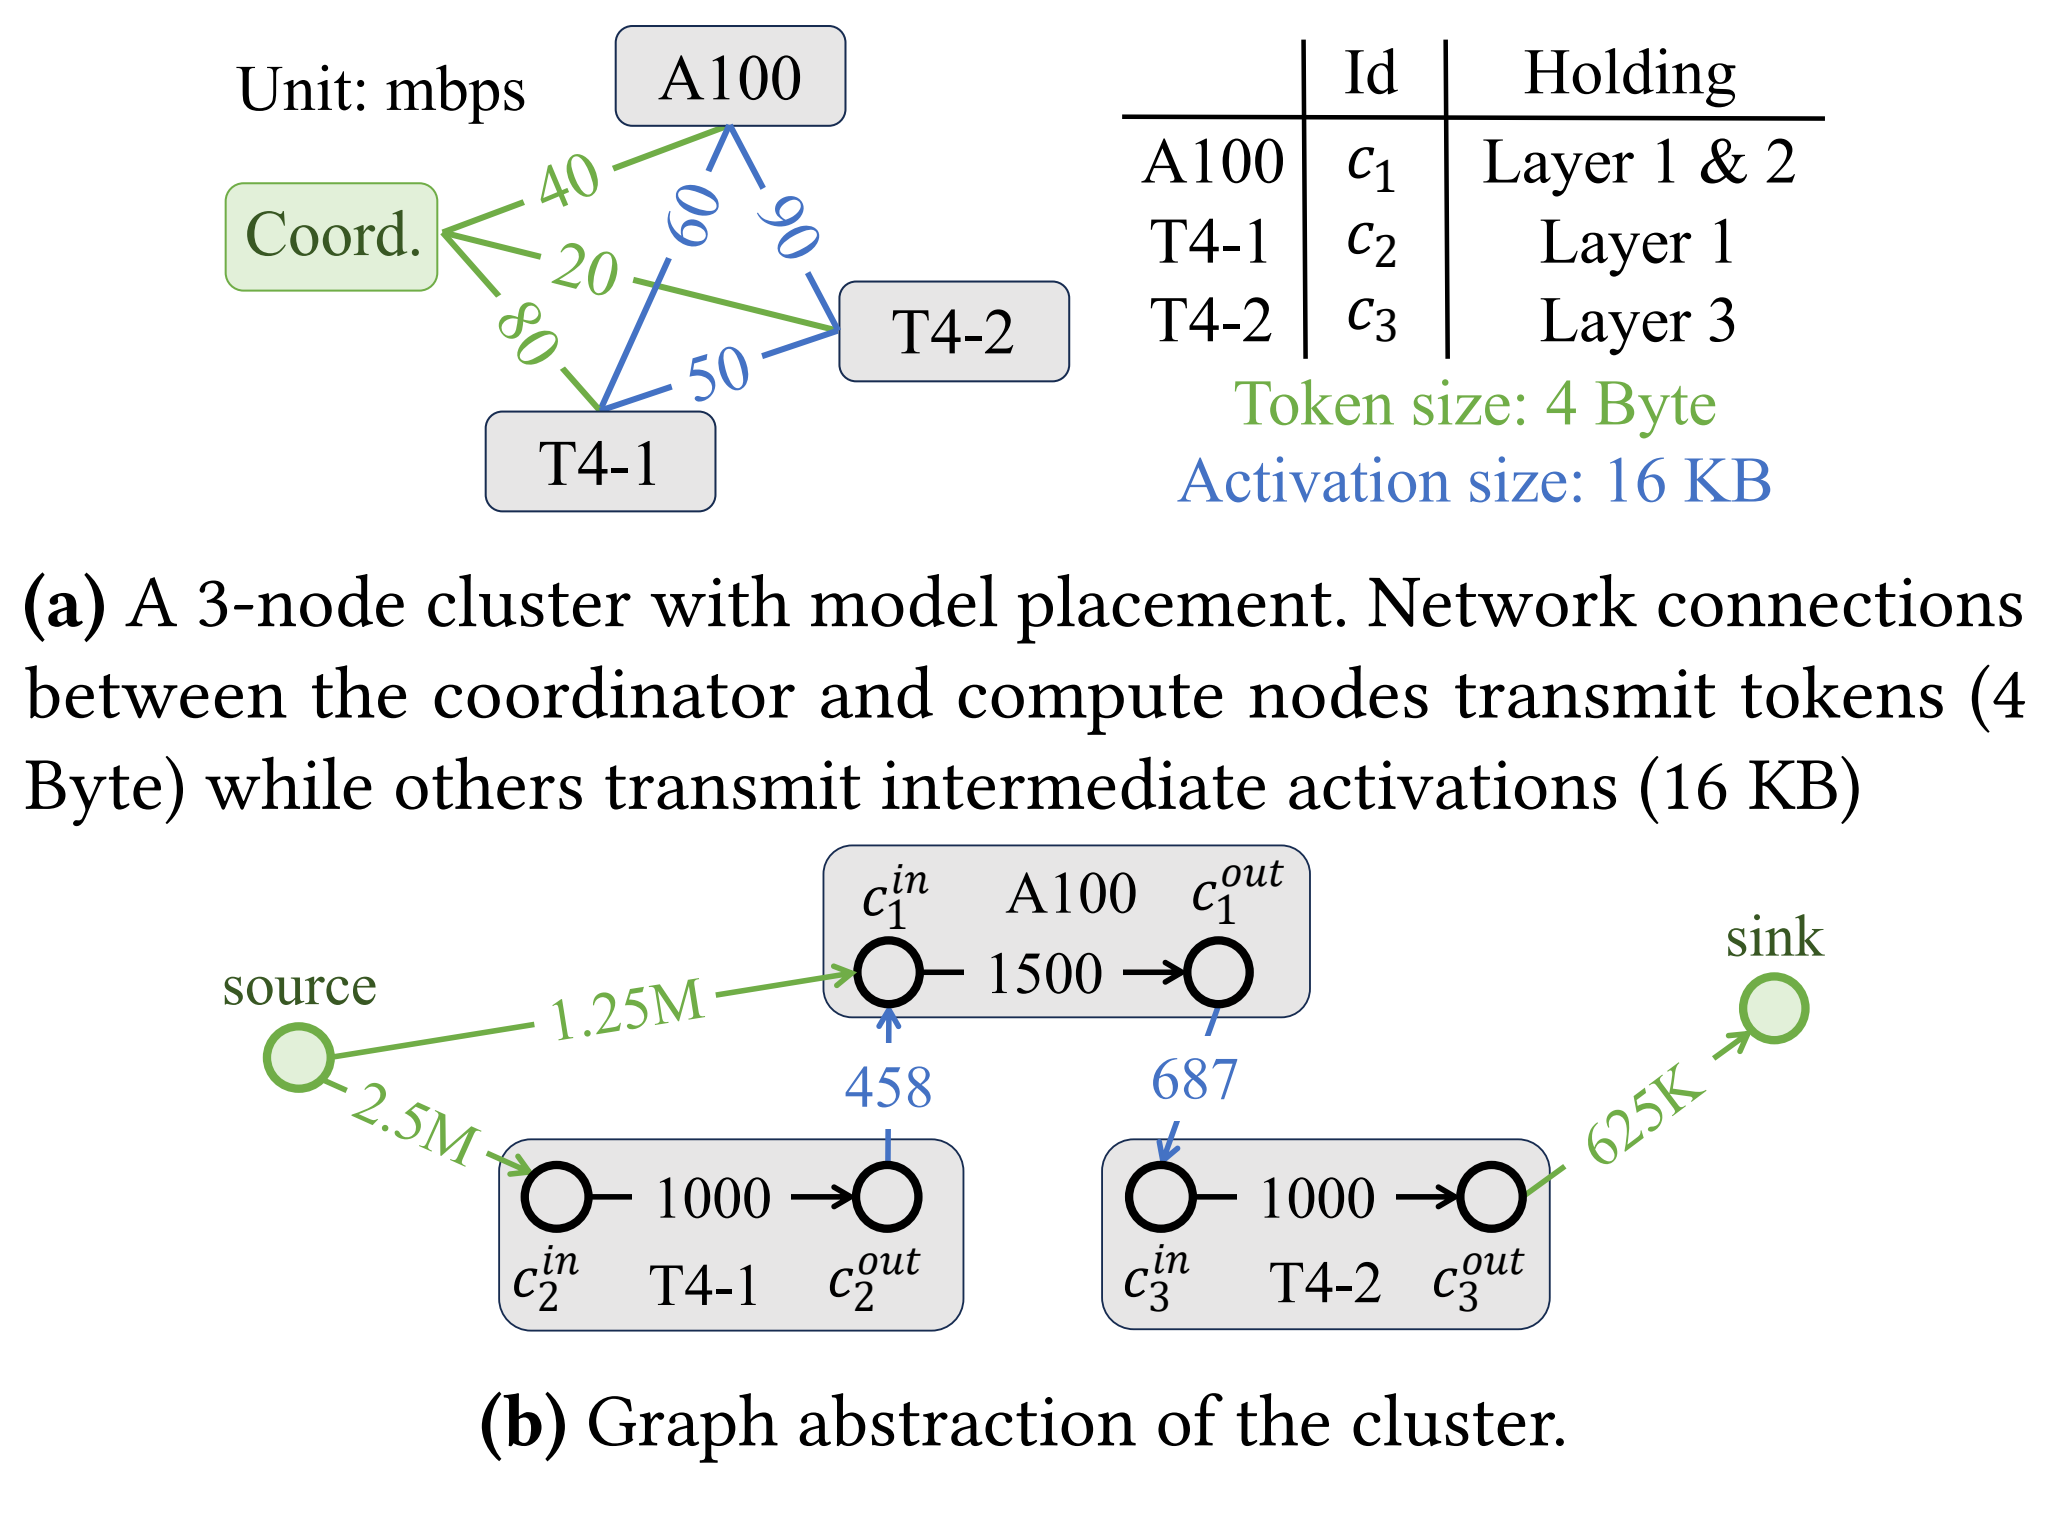
\includegraphics[width=\linewidth,trim=0 980bp 0 0,clip]{Helix/Without-Caption/Helix_Figure_02_Max_Flow_Graph_Abstraction.png}\par
 {\scriptsize\color{Muted}(a) Physical links and layer placement}\par\smallskip
 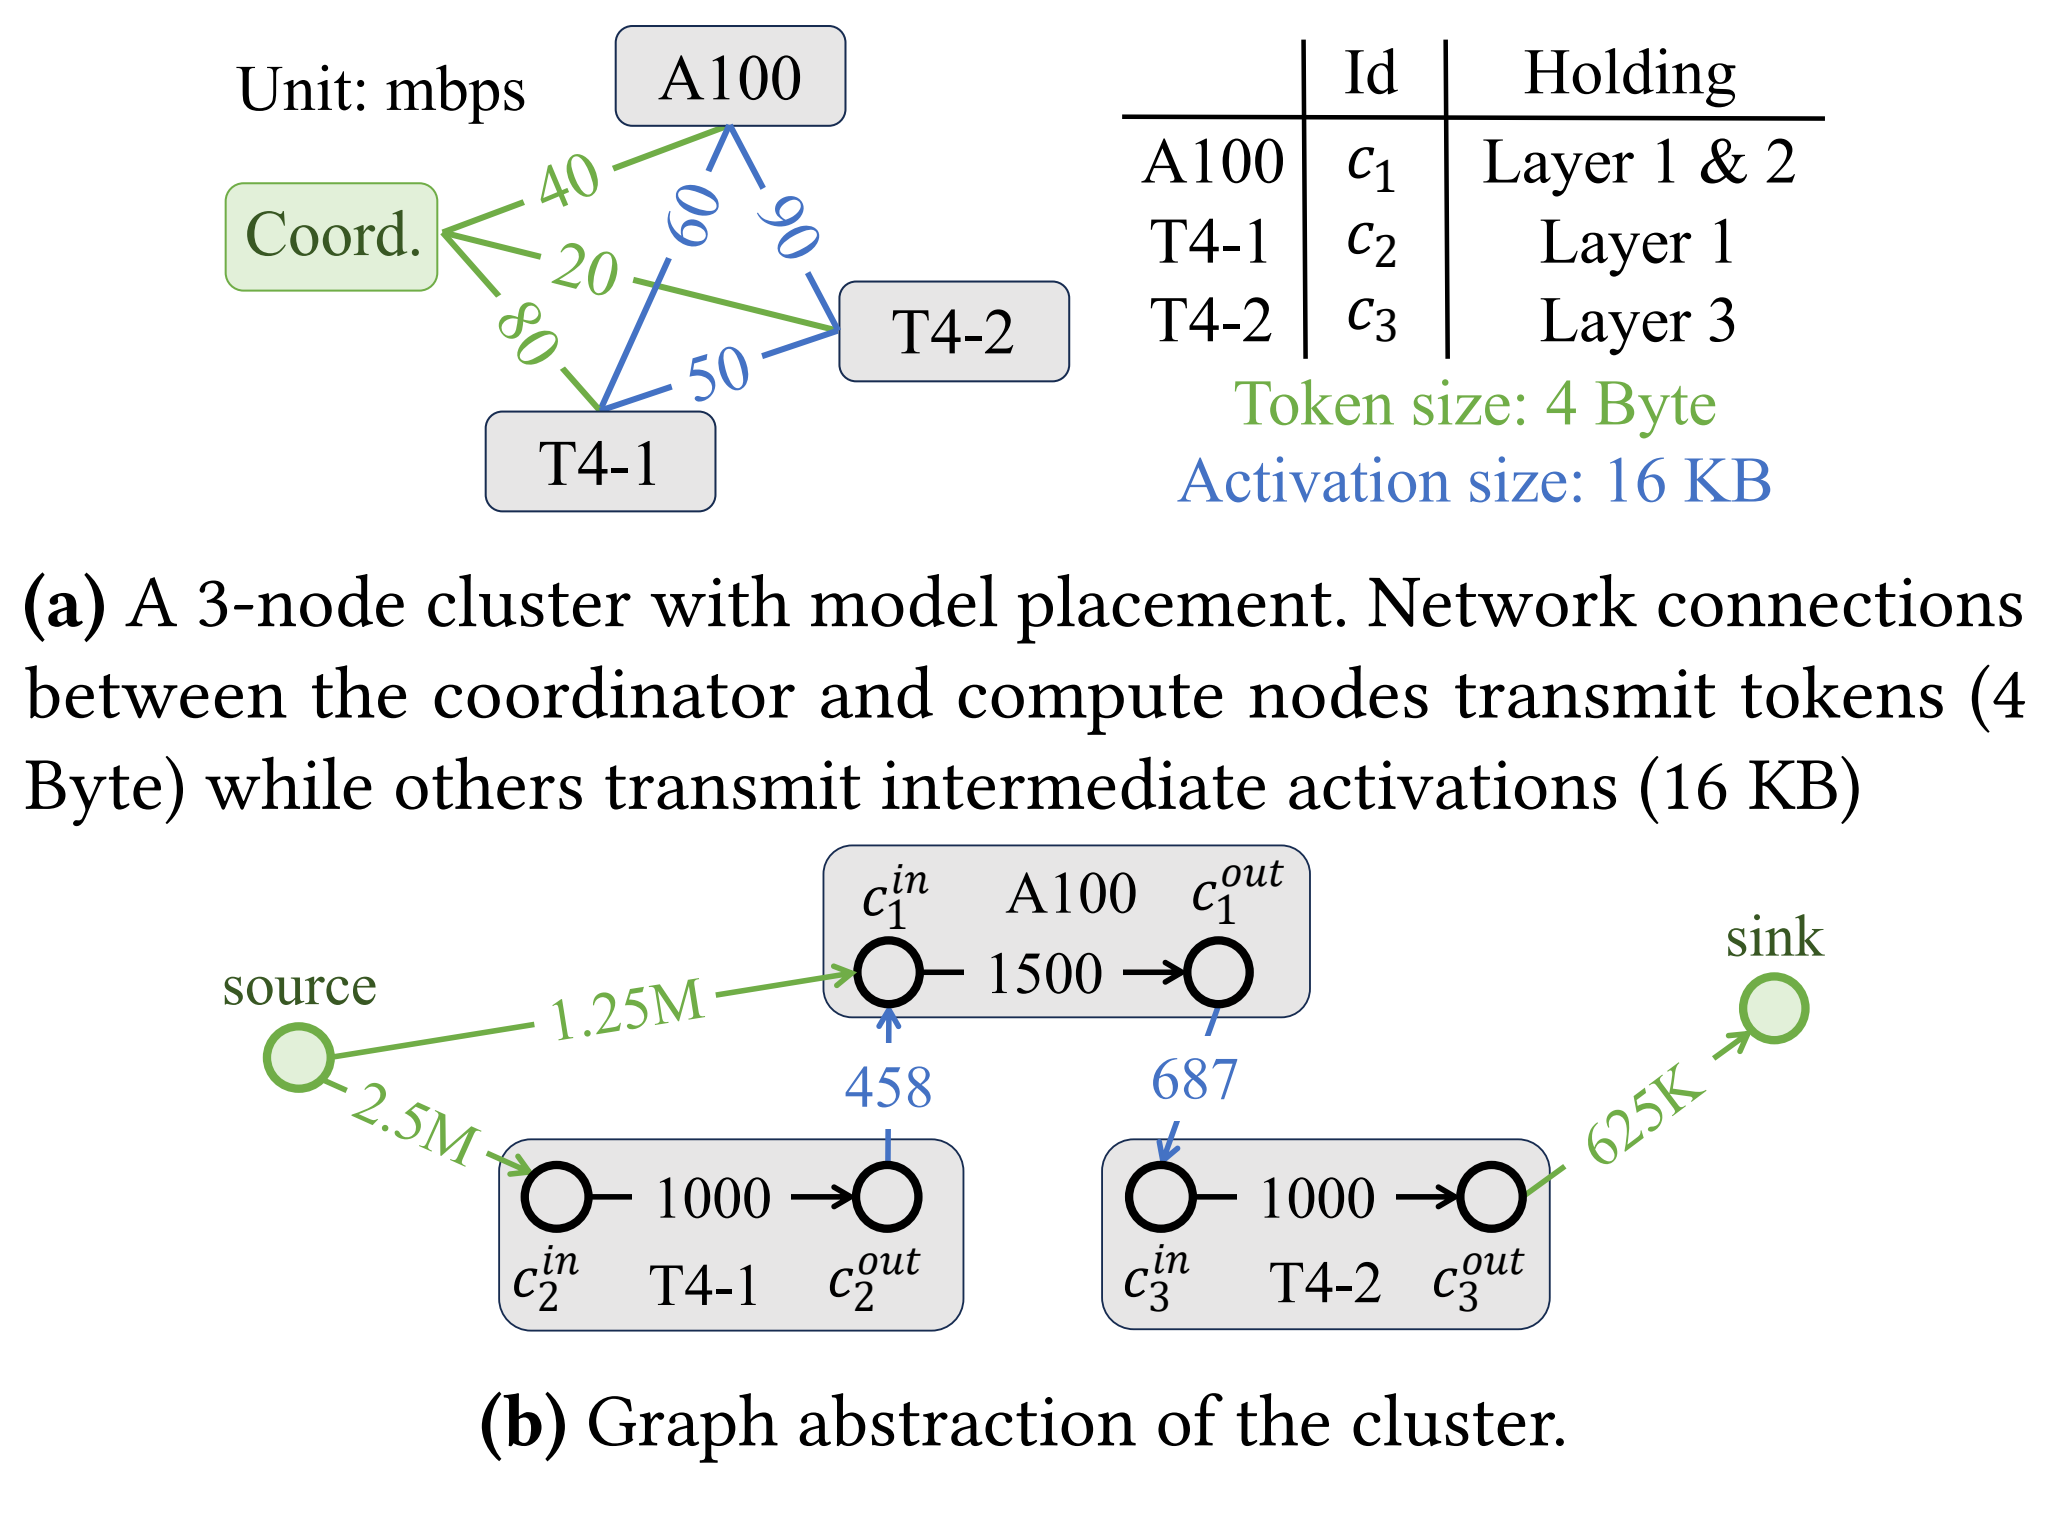
\includegraphics[width=\linewidth,trim=0 170bp 0 840bp,clip]{Helix/Without-Caption/Helix_Figure_02_Max_Flow_Graph_Abstraction.png}\par
 {\scriptsize\color{Muted}(b) Capacities in tokens/s}\par}}
\begin{document}
\section{Main}
\begin{frame}[c,label=M01]{Helix}
\vspace*{\fill}
\relax
{\LARGE\bfseries Serving Large Language Models over\par\medskip Heterogeneous GPUs and Network via Max-Flow\par}
\bigskip
{\large Joint placement and per-request scheduling}\par\bigskip
Yixuan Mei, Yonghao Zhuang, Xupeng Miao, Juncheng Yang,\\ Zhihao Jia, Rashmi Vinayak\par
{\color{Muted}Carnegie Mellon University --- ASPLOS 2025}\par\bigskip
\textbf{Research meeting: 4 November 2026}\\
Yu-Jui Liang\quad Advisor: Hsiang-Yun Cheng\\
National Taiwan University / Academia Sinica
\slidenote{title page}{\nav{INDEX}{Discussion Index} }
\end{frame}

\begin{frame}[c,label=M02]{Why Do We Need Helix?}
\vspace*{\fill}
\meta{Mixed GPU speeds and memory capacities interact with slow inter-region links.}\figureplaceholder{Helix/Without-Caption/Helix_Figure_01_Model_Placement_Examples.png}{4.8cm}{Figure 1}

\bigskip
\point{Equal layer counts}{Slow stages limit the whole pipeline.}
\point{Balanced computation}{Every request can still cross a congested network cut.}
\point{Joint placement and routing}{Local execution can reduce traffic across that cut.}
\slidenote{Secs.~3--4.2, Fig.~1 (illustrative cluster)}{\nav{B03}{Motivation Details} }
\end{frame}

\begin{frame}[c,label=M03]{What Does Helix Optimize?}
\vspace*{\fill}
\point{Placement $\Psi$}{Joint MILP chooses contiguous layer ranges for GPU nodes under memory constraints.}
\point{Capacity $c_{uv}(\Psi)$}{GPU profiling, network bandwidth, and placement determine valid graph edges and capacity limits.}
\point{Flow $f_{uv}$}{MILP jointly optimizes flow allocation with placement to maximize aggregate serving throughput.}
\[
  \max_{\Psi,f}\;\sum_i f_{\mathrm{source},i}
  \qquad \text{subject to}\quad 0\le f_{uv}\le c_{uv}(\Psi)
\]
\centering Serving throughput in tokens/s\par
\par\medskip
{\small\raggedright
The throughput objective does not directly optimize latency or its percentiles:\par\smallskip
\textbf{TTFT:} Time from request submission to the first token.\\
\textbf{TPOT:} Average time per output token after the first.\\
\textbf{P95 / P99 latency:} Latency thresholds exceeded by the slowest 5\% / 1\% of requests.\par}
\slidenote{Secs.~4.3--4.4, 5.1}{\nav{B07}{Cost Model} \nav{B13}{MILP Variables} }
\end{frame}

\begin{frame}[c,label=M04]{How Does One Request Run?}
\vspace*{\fill}
\figureplaceholder{Helix/Without-Caption/Helix_Figure_03_System_Overview.png}{3.4cm}{Figure 3}

\vspace{.12cm}
\begin{tabularx}{\textwidth}{@{}lX@{}}
\textbf{Offline planning} & Profile GPU / network resources, jointly solve placement and flow, and load model weights.\\[.12cm]
\textbf{Online scheduling} & On arrival, the coordinator checks estimated KV capacity and uses optimized flow weights in IWRR to select one valid pipeline.\\[.12cm]
\textbf{Pipeline execution} & Workers execute assigned layers in order, forward activations, and return the output token to the coordinator.\\[.12cm]
\textbf{Decode reuse} & Later tokens reuse the request's pipeline and local KV caches. MILP is not rerun per request or token.\\
\end{tabularx}
\slidenote{Secs.~4--5, Fig.~3; lifecycle synthesis}{\nav{B18}{Runtime Details} \nav{B22}{KV Cache} }
\end{frame}

\begin{frame}[c,label=M05]{How Does Max Flow Model Serving?}
\vspace*{\fill}
\begin{columns}[c,onlytextwidth]\begin{column}{.36\textwidth}
\point{Node splitting}{$c^{in}\to c^{out}$ limits compute throughput.}
\point{Network edges}{Bandwidth / payload gives tokens/s.}
\point{Source and sink}{The coordinator injects and collects tokens.}
\point{Conservation}{Flow enters and leaves each compute node at the same rate.}
\end{column}\begin{column}{.62\textwidth}\flowpanels
\end{column}\end{columns}
\par\smallskip{\small For fixed $\Psi$, $F(\Psi)=\operatorname{MaxFlow}(G(\Psi))$ models steady-state throughput.\\
The next slide jointly optimizes placement and flow.}\par
\slidenote{Sec.~4.3, Fig.~2}{\nav{B12}{Worked Cost Model} }
\end{frame}

\begin{frame}[c,label=M06]{How Does MILP Decide Placement?}
\vspace*{\fill}
\[
 \max\sum_i f_{\mathrm{source},i}
\]
{\centering\small Find the placement that supports the highest aggregate serving throughput,\par
jointly optimizing placement and flow.\par}
\medskip
{\small
\point{\hyperlink{B14}{\underline{1. Placement and memory}}}{Assign each GPU a contiguous layer range that fits its memory budget.}
\point{\hyperlink{B15}{\underline{2. Flow conservation}}}{Keep incoming and outgoing token rates equal at every worker.}
\point{\hyperlink{B15}{\underline{3. Compute capacity}}}{Limit each GPU's token rate to its profiled processing capacity.}
\point{\hyperlink{B16}{\underline{4. Connectivity}}}{Allow only hops that continue through model layers in order, from the first layer to the last.}
\point{\hyperlink{B16}{\underline{5. Network capacity}}}{Keep traffic on each valid link within its bandwidth-based token rate.}
}
{\small Pruning and timed solving produce feasible plans without always proving global optimality.}\par
\slidenote{Secs.~4.4--4.6, 6.2}{\nav{B13}{MILP Variables} \nav{B17}{Solver Settings} }
\end{frame}

\begin{frame}[c,label=M07]{How Does Runtime Scheduling Work?}
\vspace*{\fill}
\meta{IWRR = interleaved weighted round-robin. All path selection runs at the coordinator.}\figureplaceholder{Helix/Without-Caption/Helix_Figure_04_Per_Request_Pipeline_Scheduling.png}{4.05cm}{Figure 4}

\smallskip
\small\point{Weights}{Use optimized edge flows, rather than raw link capacities.}
\point{Selection}{Walk the valid graph using each vertex's IWRR state, after KV masking.}
\point{Reuse}{Interleaving avoids bursts. A request reuses its pipeline across decode steps.}
\slidenote{Sec.~5.1, Fig.~4}{\nav{B20}{IWRR Scheduling} }
\end{frame}

\begin{frame}[c,label=M08]{How Are Weights and KV Cache Managed?}
\vspace*{\fill}
\meta{Illustrative example: six layers, numbered 0--5. Half-open ranges.}
\begin{center}
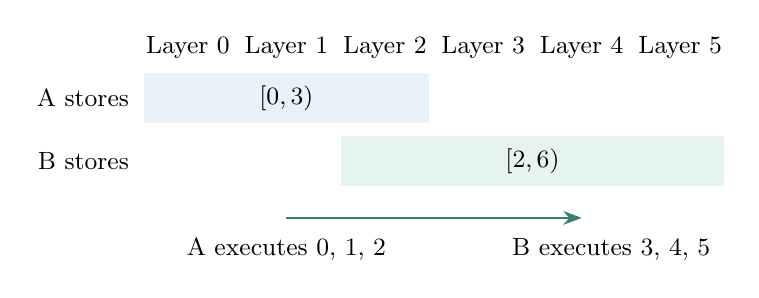
\begin{tikzpicture}[x=1.25cm,y=.8cm,every node/.style={font=\small}]
\foreach \x in {0,...,5}{\node at (\x,1.2) {Layer \x};}
\node[anchor=east] at (-.5,.4) {A stores};
\fill[SoftBlue] (-.45,0) rectangle (2.45,.8);
\node at (1,.4) {$[0,3)$};
\node[anchor=east] at (-.5,-.6) {B stores};
\fill[SoftMint] (1.55,-1) rectangle (5.45,-.2);
\node at (3.5,-.6) {$[2,6)$};
\draw[-{Stealth},thick,Accent] (1,-1.5) -- (4,-1.5);
\node at (1,-2) {A executes 0, 1, 2};
\node at (4.3,-2) {B executes 3, 4, 5};
\end{tikzpicture}
\end{center}
\point{Overlapping weights}{B stores layer 2, but this request skips it on B.}
\point{KV ownership}{Keep request-specific KV for the layers actually executed on each worker.}
\point{KV-aware selection}{Mask workers whose estimated KV usage exceeds the high-water mark, then apply flow-weighted IWRR to the remaining candidates.}
\slidenote{Secs.~4.4, 5.1--5.2, 6.1; illustrative diagram}{\nav{PARTIAL}{Partial Inference} \nav{B22}{KV Cache} }
\end{frame}

\begin{frame}[c,label=M09]{How Is Helix Evaluated?}
\vspace*{\fill}
\begin{tabularx}{\textwidth}{@{}lXX@{}}\toprule
Setting & Hardware / network & Evidence\\\midrule
Single cluster & 4 A100 + 8 L4 + 12 T4; 10 Gb/s & 24-node prototype + simulator validation\\[.2cm]
Geo-distributed & Same 24 nodes, 3 clusters; mean 100 Mb/s, 50 ms across clusters & Simulation\\[.2cm]
Higher heterogeneity & 42 nodes, 7 types including multi-GPU nodes & Simulation\\\bottomrule
\end{tabularx}
\bigskip
\point{Models and workload}{FP16 LLaMA-1 30B / LLaMA-2 70B; filtered Azure Conversation trace.}
{\small Remove requests with input $>2048$ or output $>1024$ tokens.\\
Retain 16,657 requests: mean input 763 tokens, mean output 232 tokens.}\par\medskip
\point{Metrics}{Offline saturation: decode tokens/s. Online: throughput plus prompt / decode latency.}
\slidenote{Secs.~6.1--6.2}{\nav{B24}{Experiment Setup} \nav{B25}{Workload} }
\end{frame}

\begin{frame}[c,label=BASELINES]{What Does Helix Compare Against?}
\vspace*{\fill}
\small
\begin{tabularx}{\textwidth}{@{}lXX@{}}\toprule
Method & Core approach & Comparison scope\\\midrule
\textbf{Helix} & Joint MILP placement and flow; flow-weighted IWRR & Jointly accounts for GPU and network limits.\\[.18cm]
\textbf{Swarm} & Heuristic placement and scheduling adapted from heterogeneous training & End-to-end serving baseline, reimplemented in Helix.\\[.18cm]
\textbf{SP} & Separate model pipelines for each GPU type & End-to-end serving baseline; restricts mixing GPU types within a pipeline.\\[.18cm]
\textbf{Petals} & Decentralized placement heuristic & Placement-only baseline; no end-to-end serving comparison.\\\bottomrule
\end{tabularx}\par
\medskip
\textbf{Placement ablation:} Fix the Helix scheduler and vary placement (Helix / Swarm / Petals) to isolate placement gains.\par
\slidenote{Secs.~2.2, 6.2, 6.6, Fig.~9}{\nav{SETUP}{Baseline Details} \nav{B29}{Placement Ablation} }
\end{frame}

\begin{frame}[c,label=M10]{Does Helix Improve Single-Cluster Serving?}
\vspace*{\fill}
\meta{24-node prototype and simulator check. FP16 30B / 70B. Baselines: SP and Swarm.}\figureplaceholder{Helix/Helix_Figure_06_Single_Cluster_Results.png}{5.05cm}{Figure 6}
\par\smallskip
{\small\raggedright
\textbf{Offline:} Supply enough requests to saturate the cluster; measure achievable throughput.\par\smallskip
\textbf{Online:} Azure Conversation arrivals average 75\% of peak throughput; the cluster is not always saturated.\par}
\slidenote{Secs.~6.2--6.3, Fig.~6}{\nav{B26}{All Ratios} \nav{FIG6}{Full Figure} }
\end{frame}

\begin{frame}[c,label=M11]{Does Helix Work Across Regions?}
\vspace*{\fill}
\meta{Simulation: 24 nodes in 3 clusters; mean inter-cluster 100 Mb/s and 50 ms.}\figureplaceholder{Helix/Helix_Figure_07_Geo_Distributed_Cluster_Results.png}{3.6cm}{Figure 7}

\medskip\small
\point{Throughput}{Helix achieves higher throughput than both baselines across regions, with larger gains over SP for the larger model.}
\point{Latency}{Helix improves latency over Swarm, but does not consistently outperform both baselines.}
\slidenote{Sec.~6.4, Fig.~7}{\nav{B27}{Geo Details} \nav{FIG7}{Full Figure} }
\end{frame}

\begin{frame}[c,label=M12]{What Happens with More GPU Types?}
\vspace*{\fill}
\meta{42-node simulation; LLaMA-2 70B FP16; Swarm, SP, and SP+ baselines.}\figureplaceholder{Helix/Without-Caption/Helix_Figure_08_High_GPU_Heterogeneity_Results.png}{4.85cm}{Figure 8}
\par\medskip{\small Helix maintains higher throughput with greater GPU heterogeneity, but does not consistently improve latency.}\par
\slidenote{Sec.~6.5, Fig.~8}{\nav{B28}{42-node Details} }
\end{frame}

\begin{frame}[c,label=M13]{Where Do the Gains Come From: Placement?}
\vspace*{\fill}
\meta{Offline LLaMA-2 70B. Fixed Helix scheduler; vary placement only.}\figureplaceholder{Helix/Without-Caption/Helix_Figure_09_Model_Placement_Comparison.png}{4.5cm}{Figure 9}

\bigskip
{\small With the same Helix scheduler, Helix's placement achieves the highest throughput and keeps GPUs more fully utilized.}\par
\slidenote{Sec.~6.6, Fig.~9}{\nav{B29}{Ablation Details} \nav{FIG9}{Graph Detail} }
\end{frame}

\begin{frame}[c,label=M14]{Where Do the Gains Come From: Scheduling?}
\vspace*{\fill}
\meta{Offline LLaMA-2 70B. Fixed Helix placement; vary scheduler only.}\figureplaceholder{Helix/Without-Caption/Helix_Figure_10_Request_Scheduling_Comparison.png}{4.3cm}{Figure 10}

\bigskip
{\small MILP placement and scheduling work together: even with optimized placement, Helix's flow-aware IWRR scheduler reduces network congestion and further improves throughput.}\par
\slidenote{Sec.~6.7, Fig.~10}{\nav{B30}{Ablation Details} \nav{FIG10}{Graph Detail} }
\end{frame}

\begin{frame}[c,label=M15]{Conclusion \& Discussion}
\vspace*{\fill}
{\small
\textbf{\color{Accent}Contribution --- Joint Placement and Scheduling}\par
Max-flow models heterogeneous GPU compute and network capacities. MILP jointly optimizes layer placement and flow; IWRR maps the solution to per-request pipelines.\par\medskip
\textbf{\color{Accent}Evidence --- Both Components Improve Throughput}\par
\begin{itemize}
  \setlength{\itemsep}{0pt}
  \item 24-node prototype: $1.69\times$ online throughput vs. SP (70B).
  \item Geo-distributed and 42-node evaluations use simulation.
  \item Ablations confirm gains from both placement and scheduling.
\end{itemize}
\smallskip
\textbf{\color{Accent}Trade-off --- Throughput vs. Latency}\par
Better utilization of slower GPUs improves aggregate throughput, but may increase decode latency.\par\medskip
\textbf{\color{Accent}Limitations --- Static Planning}\par
Offline placement and profiled capacities; average-length KV estimates; finite MILP solving budget.\par\medskip
\textbf{\color{Accent}Research Questions}\par
\begin{itemize}
  \setlength{\itemsep}{0pt}
  \item When should placement and flow weights adapt to workload or network changes?
  \item How can throughput optimization incorporate latency SLOs and power constraints?
\end{itemize}
}
\slidenote{Secs.~4--6, Figs.~6--10. Research questions are proposed extensions.}{\nav{INDEX}{Discussion Index} \nav{FUTURE}{Research Directions} }
\end{frame}

\section{Discussion Index}
\begin{frame}[c,label=INDEX]{Discussion Index}
\vspace*{\fill}
\begin{tabularx}{\textwidth}{@{}lXl@{}}\toprule
Topic & Questions & Jump\\\midrule
A. Background & GPU heterogeneity, TP / PP / DP, placement bottlenecks & \nav{B01}{Open A}\\[.35cm]
B. Max flow / MILP & Cost units, constraints, partial inference, solver & \nav{B07}{Open B}\\[.35cm]
C. Runtime & Architecture, IWRR, KV cache, batching & \nav{B18}{Open C}\\[.35cm]
D. Evidence & Settings, trace, complete figures, all ratios & \nav{B24}{Open D}\\[.35cm]
E. Discussion & Static plans, latency, validity, future work & \nav{B33}{Open E}\\\bottomrule
\end{tabularx}
\bigskip
Every backup has a numbered \textbf{Main} return link and related-topic links.\\
The footer opens this index from any page.
\back{M15}

\end{frame}

\section{A: Background}
\begin{frame}[c,label=B01]{Why Heterogeneous and Geo-Distributed Serving?}
\vspace*{\fill}
\vspace{.08cm}
  {\small\textbf{Table 3.} Datasheet properties. SXM for H100 and A100. Not measured serving throughput.}\par
  \vspace{.04cm}
  {\centering\small
  \begin{tabular}{lcccc}\toprule
    GPU & FP16 (TFLOP/s) & Memory & Bandwidth & Price (USD)\\\midrule
    H100 & 1979 & 80 GB & 3350 GB/s & 25k--40k\\
    A100 & 312 & 40 GB & 1555 GB/s & 10k--15k\\
    L4 & 242 & 24 GB & 300 GB/s & $\sim$3k\\
    T4 & 65 & 16 GB & 300 GB/s & $\sim$1k\\\bottomrule
  \end{tabular}\par}
  \vspace{.08cm}
  \begin{itemize}\small
    \setlength{\itemsep}{.16cm}
    \item Table 1: if half the memory stores parameters, LLaMA-2 70B needs 12 L4s, 7 A100s, or 4 H100s.
    \item Table 4: in one us-east window the quota was 8 A100 + 8 L4 + 16 T4, but only 16 T4s were deployed.
    \item The paper's claim: eight L4s have FP16 throughput comparable to one H100, with more memory and less power.
  \end{itemize}
  \par\smallskip{\small Scarcity, not a universal speed ranking, is why Helix aggregates mixed GPUs across regions.}\par
  \src{Sec.~1, Tables 1--4. Eight-L4 comparison is a datasheet argument.}
\back[\nav{B02}{Parallelism} \nav{B03}{Placement} \nav{B04}{Network}]{M02}
\end{frame}

\begin{frame}[c,label=B02]{Parallelism Across Nodes and GPUs}
\vspace*{\fill}
\point{Tensor parallelism (TP)}{Split a layer across GPUs inside one node. Each layer requires two collectives, making high-latency cross-node TP expensive.}
\point{Pipeline parallelism (PP)}{Partition layers across nodes and transfer activations between stages. Equal cuts can leave faster GPUs waiting.}
\point{Data parallelism (DP)}{Replicas process different requests. A replica may itself use TP / PP.}
\point{Petals}{A joining node greedily takes the least-loaded stage in a decentralized volunteer system.}
\point{Swarm}{Even model partitions and next-stage routing using real-time throughput. Helix reimplements this training method as an inference baseline.}
\src{Secs.~2.2--3, 6.2}\back{M02}
\end{frame}

\begin{frame}[c,label=B03]{Uniform Model Placement Is Sub-Optimal}
\vspace*{\fill}
\vspace{.04cm}
  \figureplaceholder{Helix/Without-Caption/Helix_Figure_01_Model_Placement_Examples.png}{4.4cm}{Figure 1}
  {\centering\hint{Fig.~1a--c. Illustrative example, not the 24-node cluster. Order: A100 $>$ L4 $>$ T4.}\par}
  \vspace{.02cm}
  {\small (b) Equal cuts still wait on the slower stage. (c) Balanced FLOPs still cross the slow inter-region link on every request.}

  \src{Sec.~3.1 and Sec.~4.2, Fig.~1a--c. PDF p.~4.}
\back[\nav{B04}{Network Congestion}]{M02}
\end{frame}

\begin{frame}[c,label=B04]{Network-Unaware Routing Creates Congestion}
\vspace*{\fill}
\vspace{.04cm}
  \figureplaceholder{Helix/Without-Caption/Helix_Figure_01_Model_Placement_Examples.png}{4.4cm}{Figure 1}
  {\centering\hint{Fig.~1c--d. Same illustrative cluster as the previous slide.}\par}
  \vspace{.04cm}
  \begin{itemize}\small
    \setlength{\itemsep}{.16cm}
    \item In (c) the A100's send side congests: every activation still crosses into Region 2.
    \item (d) runs two T4s beside the A100, so less traffic uses the slow link.
    \item Partition, placement, and routing have to be chosen together.
  \end{itemize}

  \src{Sec.~4.2, Fig.~1c--d. PDF p.~4.}
\back{M02}
\end{frame}

\section{B: Max Flow and MILP}
\begin{frame}[c,label=B05]{Helix Design Requirements}
\vspace*{\fill}
\point{Placement}{One cluster plan assigns each node a contiguous range of layers, respecting memory and the network.}
\point{Throughput estimate}{Measure the token rate that can flow from the coordinator through workers and back.}
\point{Scheduling}{Choose a pipeline per request. Different requests can share workers instead of using disjoint fixed pipelines.}
\par\smallskip{\small Offline placement and online scheduling share the graph but run at different timescales.}\par
\medskip
KV-cache admission is a runtime mask. Table 6 does not add a separate KV-byte objective or variable to the placement MILP.
\src{Secs.~3--5}\back{M03}
\end{frame}

\begin{frame}[c,label=B06]{Helix System Overview}
\vspace*{\fill}
\vspace{.02cm}
  \figureplaceholder{Helix/Without-Caption/Helix_Figure_03_System_Overview.png}{3.4cm}{Figure 3}

  \vspace{.04cm}
  \begin{columns}[T,onlytextwidth]
    \begin{column}{.49\textwidth}
      {\small\begin{itemize}\setlength{\itemsep}{.03cm}
        \item Profiler collects cluster info. The planner solves placement once per cluster.
        \item A new request gets a pipeline and is sent to the first node only.
      \end{itemize}}
    \end{column}
    \begin{column}{.49\textwidth}
      {\small\begin{itemize}\setlength{\itemsep}{.03cm}
        \item Each node runs its layers and forwards the activation.
        \item The last node returns the token. The next token reuses the same pipeline.
      \end{itemize}}
    \end{column}
  \end{columns}
  \par\smallskip{\small The coordinator owns placement and scheduling. Compute nodes do not re-plan the route.}\par
  \src{Sec.~5, Fig.~3. PDF p.~7.}
\back{M04}
\end{frame}

\begin{frame}[c,label=B07]{From Model Placement to a Flow Network}
\vspace*{\fill}
\vspace{.10cm}
  \begin{itemize}\small
    \setlength{\itemsep}{.08cm}
    \item A cluster has one coordinator \(h\) and compute nodes \(C\). A multi-GPU machine is one logical node: compute and VRAM are summed.
    \item Placement \(\Psi\) gives each node a contiguous layer range. Scheduling \(\phi\) gives each request an ordered node sequence.
    \item A common score keeps only the slowest stage, \(\min_i \sum_j \mathrm{capacity}(j)\cdot \mathbf{1}[i\in\Psi(j)]\).
    \item Fig.~1c has balanced stage FLOPs and is still limited by the wide-area link. The min-stage score cannot see that.
  \end{itemize}
  \par\smallskip{\small Helix scores a placement by the max flow of a graph, in tokens per second.}\par
  \src{Sec.~4.1--4.2. The min-stage formula is the paper's description of prior heuristics.}
\back[\nav{M03}{Main 3} \nav{B05}{Design} \nav{B08}{Graph} \nav{B09}{Compute} \nav{B10}{Network} \nav{B11}{Throughput}]{M05}
\end{frame}

\begin{frame}[c,label=B08]{Max-Flow Graph Abstraction}
\vspace*{\fill}
\vspace{.02cm}
  \begin{columns}[c,onlytextwidth]
    \begin{column}{.36\textwidth}
      {\small\begin{itemize}\setlength{\itemsep}{.08cm}
        \item Each compute node becomes \(c^{\mathrm{in}}\rightarrow c^{\mathrm{out}}\).
        \item The coordinator becomes the source and the sink.
        \item An edge capacity is how many tokens may cross it per second.
        \item Max flow from source to sink is the serving throughput of this placement.
      \end{itemize}}

    \end{column}
    \begin{column}{.62\textwidth}
      \flowpanels
      {\centering\hint{Fig.~2. Capacities are tokens/s.}\par}
    \end{column}
  \end{columns}
  \src{Sec.~4.3, Fig.~2. PDF p.~4.}
\back[\nav{B09}{Compute} \nav{B10}{Network} \nav{B11}{Throughput}]{M05}
\end{frame}

\begin{frame}[c,label=B09]{Modeling Compute Capacity}
\vspace*{\fill}
\point{Split each worker}{$c^{in}\to c^{out}$ is the internal edge through which all assigned flow must pass.}
\[
 c_{\mathrm{node}}=\min\{\text{profiled compute tokens/s},\ \text{node network tokens/s}\}
\]
\point{Profile the layer count}{$T_j$ is the measured token rate for a node holding $j$ layers. MILP binaries select the appropriate rate.}
\point{Coordinator}{Source and sink inject and collect tokens, without a GPU compute edge.}
\par\smallskip{\small Datasheet TFLOP/s motivate heterogeneity; measured token rates parameterize the serving model.}\par
\src{Secs.~4.3--4.4, Constraint 3}\back{M05}
\end{frame}

\begin{frame}[c,label=B10]{Modeling Network Capacity}
\vspace*{\fill}
\vspace{.08cm}
  {\small A link is valid only in one of three cases:}\par
  \vspace{.08cm}
  \begin{enumerate}\small
    \setlength{\itemsep}{.06cm}
    \item Coordinator \(\rightarrow\) a node that holds the first layer. Payload is a token (Fig.~2 uses 4 bytes).
    \item A node that holds the last layer \(\rightarrow\) coordinator. Payload is again a token.
    \item Node \(i\rightarrow\) node \(j\) when \(j\) holds the layers needed immediately after \(i\). Payload is an activation (Fig.~2 uses 16 KB).
  \end{enumerate}
  \vspace{.08cm}
  \[
    \text{capacity (tokens/s)}=\frac{\text{profiled average bandwidth}}{\text{bytes per token or activation}}.
  \]
  {\small The formula is the paper's rule. The byte sizes above are the Fig.~2 annotations, not universal constants.}\par
  \par\smallskip{\small Activations cost far more tokens of budget than the final output token, so wide-area links saturate first.}\par
  \src{Sec.~4.3. Bandwidth is a one-time average, not a runtime measurement.}
\back{M05}
\end{frame}

\begin{frame}[c,label=B11]{Why Max Flow Represents Serving Throughput}
\vspace*{\fill}
\vspace{.10cm}
  \begin{itemize}\small
    \setlength{\itemsep}{.08cm}
    \item One unit of flow is one token that can pass a node or a link in one second.
    \item Conservation forces tokens into \(c^{\mathrm{in}}\) to leave through \(c^{\mathrm{out}}\).
    \item Helix computes the source--sink max flow with preflow-push. That value is the placement's max serving throughput.
    \item The model is a steady token rate. It does not output prompt latency, decode latency, or a percentile.
    \item Early stopping uses aggregate compute capacity normalized by total model layers (token-layer work/s divided by layers).
  \end{itemize}

  \src{Sec.~4.3 and the early-stop remark in Sec.~4.5.}
\back{M05}
\end{frame}

\begin{frame}[c,label=B12]{Worked Three-Node Example}
\vspace*{\fill}
\begin{columns}[c,onlytextwidth]
\begin{column}{.48\textwidth}
\small
\textbf{Placement}\par\medskip
A100: layers 1--2.\\ T4-1: layer 1. T4-2: layer 3.\par\medskip
\textbf{Activation link}\par
\[
 \frac{60\times10^6\ \mathrm{bits/s}}{16\times1024\times8\ \mathrm{bits/token}}
 \approx458\ \mathrm{tokens/s}
\]
\textbf{Interpretation}\par\medskip
The KiB interpretation matches Fig.~2's rounded capacities. These payload sizes are example values.\par\medskip

\end{column}
\begin{column}{.50\textwidth}\flowpanels\end{column}
\end{columns}
\par\smallskip{\small Activation transfers constrain the flow even when token-sized links are fast.}\par
\src{Sec.~4.3, Fig.~2; unit conversion is illustrative.}\back[\nav{B08}{Graph} \nav{B09}{Compute} \nav{B10}{Network} \nav{B11}{Throughput}]{M05}
\end{frame}

\begin{frame}[c,label=B13]{MILP Variables and Objective}
\vspace*{\fill}
\vspace{.06cm}
  {\centering\small
  \begin{tabular}{lll}\toprule
    Symbol & Role & Meaning\\\midrule
    \(s_i\) & integer & first layer on node \(i\)\\
    \(b_{ij}\) & binary & node \(i\) holds exactly \(j\) layers\\
    \(f_{i,j}\) & real & flow from \(i\) to \(j\), in tokens/s\\
    \(d_{i,j}\) & binary & whether link \((i,j)\) is valid\\
    \(\mathit{cond}\) & binary & auxiliaries that linearize overlap\\\bottomrule
  \end{tabular}\par}
  \vspace{.08cm}
  {\small \(e_i=s_i+\sum_j j\,b_{ij}\). Node \(i\) holds the half-open range \([s_i,e_i)\). \(k\) is the most layers that fit on that GPU.}\par
  \vspace{.06cm}
  \[
    \max \sum_i f_{\mathrm{source},i}
  \]
  \par\smallskip{\small The objective maximizes coordinator outflow. Table 5 groups the variable counts as linear in \(|C|\) or \(|E|\).}\par
  \src{Sec.~4.4, Tables 5--6. Notation here is compacted from the paper.}
\back[\nav{M03}{Main 3} \nav{B14}{Placement} \nav{B15}{Flow / Compute} \nav{B16}{Network}]{M06}
\end{frame}

\begin{frame}[c,label=B14]{Placement and Memory Constraints}
\vspace*{\fill}
\vspace{.10cm}
  {\small\textbf{Constraint 1: contiguous placement within the memory budget.}}\par
  \[
    \sum_{j=1}^{k} b_{ij}=1,
    \qquad 0\le s_i<L,
    \qquad e_i\le L.
  \]
  \begin{itemize}\small
    \setlength{\itemsep}{.16cm}
    \item Exactly one layer-count is chosen. The range must lie inside the model's \(L\) layers.
    \item Memory enters as \(k\), the maximum number of layers the GPU can hold. Table 6 has no KV-byte variable.
    \item If \(s_j<e_i<e_j\), traffic from \(i\) runs only layers \([e_i,e_j)\) on \(j\). The paper calls this partial inference.
    \item The solver may be run with partial inference disabled. Then a link is valid only when \(e_i=s_j\).
  \end{itemize}
  \par\smallskip{\small GPU memory limits how many layers are placed. KV capacity is enforced later, at schedule time.}\par
  \src{Sec.~4.4, Constraint~1, and the partial-inference remark.}
\back{M06}
\end{frame}

\begin{frame}[c,label=B15]{Flow and Compute Constraints}
\vspace*{\fill}
\vspace{.12cm}
  {\small\textbf{Constraint 2: conservation at node \(i\).}}\par
  \[
    \sum_u f_{u,i}=\sum_v f_{i,v}.
  \]
  {\small\textbf{Constraint 3: profiled inference throughput.}}\par
  \[
    \sum_u f_{u,i}\le \sum_{j=1}^{k} b_{ij}\,T_j.
  \]
  \begin{itemize}\small
    \setlength{\itemsep}{.06cm}
    \item \(T_j\) is a profiled constant: tokens per second when this node holds \(j\) layers.
    \item The binaries \(b_{ij}\) pick exactly one of those profiled rates.
    \item Flow is still also limited by the network edges on the next slide.
  \end{itemize}

  \src{Sec.~4.4, Constraints 2--3. Sums skip node \(i\) itself, as stated in the paper.}
\back{M06}
\end{frame}

\begin{frame}[c,label=B16]{Connectivity and Network Constraints}
\vspace*{\fill}
\vspace{.06cm}
  {\small\textbf{Constraint 4, compacted.} A coordinator link into \(i\) exists only if \(i\) holds the first layer:}\par
  \[
    s_i\le L\,(1-d_{\mathrm{source},i}).
    \qquad
    L\,d_{i,\mathrm{sink}}\le e_i.
  \]
  {\small Between compute nodes, \(d_{ij}=1\) only if \(s_j\le e_i<e_j\). Two auxiliary binaries linearize that test, and \(d_{ij}\le 0.5\,\mathit{cond}^{1}+0.5\,\mathit{cond}^{2}\).}\par
  \nav{LINEAR}{Full Linearization}\par
  \vspace{.06cm}
  {\small\textbf{Constraint 5: transmission throughput.}}\par
  \[
    f_{ij}\le d_{ij}\,S_{ij}.
  \]
  {\small \(S_{ij}\) is the profiled token rate of that link, from Sec.~4.3. Invalid links carry zero flow.}\par

  \src{Sec.~4.4, Constraints 4--5. The two-auxiliary form is the paper's linearization.}
\back{M06}
\end{frame}

\begin{frame}[c,label=LINEAR]{Full Connectivity Linearization}
\vspace*{\fill}
\meta{Binary $a_{ij},b_{ij}^{\mathrm{aux}}$ stand for the paper's $cond^1,cond^2$.}
\begin{align*}
 (L+1)(1-a_{ij}) &\ge s_j-e_i,\\[.12cm]
 e_j-e_i &\ge 1-(L+1)(1-b_{ij}^{\mathrm{aux}}),\\[.12cm]
 d_{ij} &\le \tfrac12 a_{ij}+\tfrac12 b_{ij}^{\mathrm{aux}},\\[.12cm]
 0\le f_{ij} &\le d_{ij}S_{ij}.
\end{align*}
An active edge requires $s_j\le e_i<e_j$. With no partial inference, require $e_i=s_j$ instead.\par\medskip
\textbf{Interpretation:} a valid connection need not carry positive flow. Link capacity bounds flow; it is not the IWRR weight.
\src{ Sec.~4.4, Table 6. Auxiliary names adapted.}\back{M06}

\end{frame}

\begin{frame}[c,label=B17]{Making the MILP Practical}
\vspace*{\fill}
\point{Pruning}{Drop slow network connections. Evaluation uses average degree 12. This restricts the search space.}
\point{Warm start}{Petals, Swarm, and SP supply feasible starting candidates; Gurobi searches for better placements.}

\point{Early stopping}{Stop near the analytic compute upper bound, or after 10 minutes without improvement. Maximum search budget: 4 hours on a 14-core CPU.}
\point{Why not relax to LP?}{Rounding start layers or layer counts can invalidate edges and radically change feasible flow.}
\point{Scaling beyond the evaluation}{Partitioning hundreds of nodes into smaller clusters is suggested, but not evaluated.}
\src{Secs.~4.5--4.6, 6.2}\back[\nav{B31}{Pruning / Warm Start} \nav{B32}{Solver Quality}]{M06}
\end{frame}

\section{C: Runtime}
\begin{frame}[c,label=B18]{Runtime Components and Control Flow}
\vspace*{\fill}
\vspace{.12cm}
  \begin{enumerate}\small
    \setlength{\itemsep}{.08cm}
    \item \textbf{Once per cluster:} profile nodes and links, solve the MILP, load each node's layer range.
    \item \textbf{On request arrival:} the coordinator's scheduler builds one pipeline and sends the request to its first node.
    \item \textbf{On each node:} run the assigned layers for the requests that arrived during the previous batch. Do not add a waiting window.
    \item \textbf{On the last node:} return the output token to the coordinator.
    \item \textbf{On the next token:} reuse that request's pipeline. Do not solve the MILP again.
  \end{enumerate}

  \src{Sec.~5 and Fig.~3. Batching details are in Sec.~5.1.}
\back[\nav{B06}{System Overview} \nav{B19}{Pipelines}]{M04}
\end{frame}

\begin{frame}[c,label=B19]{Per-Request Pipelines}
\vspace*{\fill}
\vspace{.10cm}
  \begin{itemize}\small
    \setlength{\itemsep}{.08cm}
    \item A valid pipeline runs every layer once, in order. Each stage names a node and the layers it will run.
    \item Fixed pipelines give each pipeline a disjoint set of machines.
    \item Helix lets pipelines intersect. The candidates are the source--sink paths of the placement graph.
    \item After the pipeline is chosen, a node batches every request that arrived while it ran the previous batch. There is no extra collect window.
    \item Later tokens of the same request keep that pipeline.
  \end{itemize}

  \src{Sec.~5.1. Fixed-pipeline contrast cites prior systems, including HexGen in the related work.}
\back{M07}
\end{frame}

\begin{frame}[c,label=B20]{Converting Max-Flow Weights into Scheduling}
\vspace*{\fill}
\point{Per-vertex state}{The coordinator maintains an IWRR scheduler for each vertex in the placement graph.}
\point{Candidates}{Neighbors reachable through valid directed edges. KV masking removes nodes above the estimated high-water mark.}
\point{Weights}{Use the optimized flow $f_{uv}$ on each outgoing edge. Selection frequency is proportional to that weight.}
\point{Walk}{Choose the first worker from the coordinator's state, then choose successors until the path reaches the sink.}
\point{Interleave and reuse}{Interleaving avoids bursts. Subsequent tokens retain the selected pipeline and its KV state.}
\src{Secs.~5.1--5.2, Fig.~4}\back[\nav{B19}{Pipelines} \nav{B21}{Example} \nav{B22}{KV Cache}]{M07}
\end{frame}

\begin{frame}[c,label=B21]{Pipeline Scheduling Example}
\vspace*{\fill}
\vspace{.02cm}
  \begin{columns}[c,onlytextwidth]
    \begin{column}{.46\textwidth}
      {\small\begin{itemize}\setlength{\itemsep}{.16cm}
        \item Vertices are compute nodes. An edge exists only if the MILP placement made it valid.
        \item The number on an edge is flow in the max-flow solution, not link capacity.
        \item The figure's two example pipelines are \(1\rightarrow 5\rightarrow 9\) and \(2\rightarrow 6\rightarrow 8\).
        \item Those paths can share the cluster. They are not two frozen replicas.
      \end{itemize}}

    \end{column}
    \begin{column}{.52\textwidth}
      \figureplaceholder{Helix/Without-Caption/Helix_Figure_04_Per_Request_Pipeline_Scheduling.png}{4.85cm}{Figure 4}
    \end{column}
  \end{columns}
  \src{Sec.~5.1, Fig.~4. PDF p.~8.}
\back{M07}
\end{frame}

\begin{frame}[c,label=B22]{KV-Cache Masking and Backpressure}
\vspace*{\fill}
\vspace{.12cm}
  \begin{itemize}\small
    \setlength{\itemsep}{.09cm}
    \item Each GPU has a finite VRAM budget for KV cache. Exceeding it forces offload to host memory, which the paper says significantly cuts throughput.
    \item Output length is unknown until generation ends, so the scheduler cannot know the exact KV footprint.
    \item Helix estimates each node's KV use with the average output length.
    \item A node above the high-water mark is masked out of IWRR until some of its current requests finish.
    \item The paper does not print the numeric threshold or the byte formula for that estimate.
  \end{itemize}
  \par\smallskip{\small Backpressure is a mask on the same IWRR walk. It is not a second placement solver.}\par
  \src{Sec.~5.2. ``High water mark'' is the paper's term; its value is not specified.}
\back[\nav{M04}{Main 4} \nav{M07}{Main 7} \nav{PARTIAL}{Partial Inference}]{M08}
\end{frame}

\begin{frame}[c,label=PARTIAL]{Partial Inference and Request-Specific KV}
\vspace*{\fill}
\meta{Illustrative example: six layers, numbered 0--5. Half-open ranges.}
\begin{center}
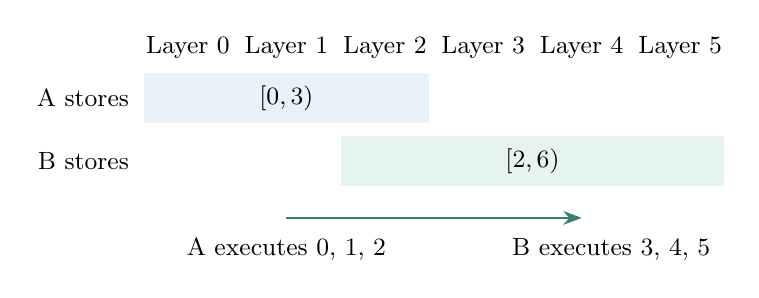
\begin{tikzpicture}[x=1.25cm,y=.8cm,every node/.style={font=\small}]
\foreach \x in {0,...,5}{\node at (\x,1.2) {Layer \x};}
\node[anchor=east] at (-.5,.4) {A stores};
\fill[SoftBlue] (-.45,0) rectangle (2.45,.8);
\node at (1,.4) {$[0,3)$};
\node[anchor=east] at (-.5,-.6) {B stores};
\fill[SoftMint] (1.55,-1) rectangle (5.45,-.2);
\node at (3.5,-.6) {$[2,6)$};
\draw[-{Stealth},thick,Accent] (1,-1.5) -- (4,-1.5);
\node at (1,-2) {A executes 0, 1, 2};
\node at (4.3,-2) {B executes 3, 4, 5};
\end{tikzpicture}
\end{center}
\point{Overlapping weights}{B stores layer 2, but this request skips it on B.}
\point{KV ownership}{Keep request-specific KV for the layers actually executed on each worker.}

\small Valid hop: $s_B\le e_A<e_B$. Strict overlap: $s_B<e_A<e_B$.\\
B runs $[e_A,e_B)$ for this request. Other paths may require different layers on B.\\
vLLM's unified page pool supports partial inference; later tokens reuse the route.
\src{ Secs.~4.4, 5.1--5.2, 6.1; illustrative example}\back{M08}

\end{frame}

\begin{frame}[c,label=B23]{Implementation and Prototype}
\vspace*{\fill}
\point{Prototype}{vLLM 0.4.0.post1, 1.5k Python + 1.7k C++ lines. Unified page pool for partial inference, ZeroMQ communication, and Gurobi placement.}
\point{Simulator}{14k Python lines model heterogeneous GPUs and networks. Geo-distributed and 42-node results use this simulator.}
\point{Validation scope}{Against the single-cluster prototype: average decode-throughput error $<5\%$, prompt-latency error $<5\%$, decode-latency error $<4\%$.}
\point{Hardware scope}{Prototype experiments use single-GPU nodes. Multi-GPU nodes use in-node TP; the 42-node simulation includes them.}
\point{Artifact scope}{Appendix A describes dummy weights. The artifact validates system performance, not generated-answer quality.}
\src{Secs.~6.1--6.3, Appendix A.2 and A.3.5}\back{M09}
\end{frame}

\section{D: Experimental Evidence}
\begin{frame}[c,label=B24]{Evaluation Methodology}
\vspace*{\fill}
\vspace{.06cm}
  {\centering\small
  \begin{tabularx}{\linewidth}{@{}lXll@{}}\toprule
    Setup & Hardware & Network & Evidence\\\midrule
    Single & 4 A100 + 8 L4 + 12 T4 & 10 Gb/s & Prototype\\[.08cm]
    Geo & Same GPUs in 3 clusters & 100 Mb/s, 50 ms & Simulation\\[.08cm]
    42-node & 7 types, single / multi-GPU nodes & Simulated & Simulation\\\bottomrule
  \end{tabularx}\par}
  \vspace{.08cm}
  \begin{itemize}\small
    \setlength{\itemsep}{.10cm}
    \item Models: LLaMA-1 30B and LLaMA-2 70B, FP16. Baselines: Swarm, and separate pipelines (SP) inside Helix.
    \item Petals is compared only as a placement (Sec.~6.6), not as an end-to-end server.
    \item Offline metric: average decode throughput, in generated tokens/s. Online adds average prompt and decode latency.
    \item Online arrivals are the Azure shape scaled to 75\% of that cluster's peak. Offline arrivals saturate the cluster.
  \end{itemize}

  \src{Sec.~6.2. The 100 Mb/s geo setting is justified by Table 7, whose pairs span 54--204 Mb/s.}
\back[\nav{B23}{Implementation} \nav{SETUP}{Baselines} \nav{B25}{Workload}]{M09}
\end{frame}

\begin{frame}[c,label=SETUP]{Hardware, Baselines, and Normalization}
\vspace*{\fill}
\small
\textbf{42 nodes:} 4 A100, 6 V100, 8 L4, 10 T4, 4 $2\times$L4, 6 $2\times$T4, 4 $4\times$T4.\par\medskip
\textbf{Geo clusters:} (4 A100), (2 L4 + 8 T4), (6 L4 + 4 T4). Measured cross-region links in Table 7 span 54--204 Mb/s; experiments simulate mean 100 Mb/s / 50 ms.\par\medskip
\textbf{Swarm:} placement and scheduler reimplemented in Helix; minimum stage count lets the weakest GPU fit one stage in half its VRAM.\par\medskip
\textbf{SP:} one replica per GPU type, implemented in Helix. \textbf{Petals:} placement only, using Helix's scheduler.\par\medskip
\textbf{Ratios:} $x\times=\mathrm{Helix\ throughput}/\mathrm{named\ baseline\ throughput}$. Percentage latency change uses that baseline's mean latency.\par\medskip
\textbf{Fig.~11:} throughput and solver-time comparisons use the paired without-pruning / default-initialization run as the reference, respectively. Fig.~12 plots an objective value and bound, not a serving-latency speedup.
\src{ Secs.~6.2, 6.5--6.9, Table 7}\back{BASELINES}

\end{frame}

\begin{frame}[c,label=B25]{Workload Characteristics}
\vspace*{\fill}
\figureplaceholder{Helix/Without-Caption/Helix_Figure_05_Azure_Conversation_Statistics.png}{3.1cm}{Figure 5}
\medskip
{\small
\textbf{Filtering:} remove input $>2048$ or output $>1024$ tokens; retain 16,657 requests.\\[.12cm]
\textbf{Mean lengths:} 763 input tokens and 232 output tokens.\\[.12cm]
\textbf{Runs:} online 30 s warmup + 30 min; offline 1 min warmup + 10 min.\\[.12cm]
\textbf{Figure:} Azure Conversation before online 75\% scaling. Latency results apply to this filtered trace.\par}
\src{Sec.~6.2, Fig.~5. PDF p.~8.}
\back{M09}
\end{frame}

\begin{frame}[c,label=FIG6]{Complete Figure 6: Single-Cluster Results}
\vspace*{\fill}
\meta{24-node prototype and simulator check. FP16 30B / 70B. Baselines: SP and Swarm.}\figureplaceholder{Helix/Without-Caption/Helix_Figure_06_Single_Cluster_Results.png}{4.8cm}{Figure 6}
\small
Top: decode tokens/s. Bottom: 30B prompt/decode, then 70B prompt/decode (s).\\
Boxes: 25--75th percentiles; whiskers: 5--95th; red: median.
\src{ Sec.~6.3, Fig.~6}\back[\nav{B26}{Detailed Ratios}]{M10}
\end{frame}

\begin{frame}[c,label=B26]{Single-Cluster Results}
\vspace*{\fill}
\vspace{.02cm}

  {\centering\hint{Fig.~6. Prototype. (a--d) decode throughput; (e--h) online latency. Box 25--75, whisker 5--95, red line = median.}\par}
  \vspace{.02cm}
  {\centering\small
  \begin{tabular}{llcccc}\toprule
    Model & Versus & Offline tput & Online tput & Prompt lat. & Decode lat.\\\midrule
    30B & SP & \(+4\%\) & \(+14\%\) & \(-2\%\) & \(+10\%\)\\
    30B & Swarm & \(2.14\times\) & \(2.07\times\) & \(-32\%\) & \(-12\%\)\\
    70B & SP & \(1.86\times\) & \(1.69\times\) & \multicolumn{2}{c}{average latency higher}\\
    70B & Swarm & \(1.94\times\) & \(2.00\times\) & \(-15\%\) & \(+16\%\)\\\bottomrule
  \end{tabular}\par}
  \vspace{.02cm}
  {\small 30B: three replicas, one GPU type each. 70B vs.\ SP: latency is higher because SP serves most requests on A100s and leaves L4/T4 idle.}\par

  \src{Sec.~6.3, Fig.~6. Pairs are offline then online. PDF p.~9.}
\back[\nav{FIG6}{Full Figure}]{M10}
\end{frame}

\begin{frame}[c,label=FIG7]{Complete Figure 7: Geo-Distributed Results}
\vspace*{\fill}
\meta{Simulation: 24 nodes in 3 clusters; mean inter-cluster 100 Mb/s and 50 ms.}\figureplaceholder{Helix/Without-Caption/Helix_Figure_07_Geo_Distributed_Cluster_Results.png}{3.6cm}{Figure 7}

\medskip\small
Left: 30B / 70B tokens/s. Right: 30B prompt/decode, then 70B prompt/decode (s).\\
H = Helix, S = Swarm; boxes 25--75th, whiskers 5--95th, red = median.
\bigskip
\point{Simulated 30B vs. Swarm}{Online prompt latency $-66\%$, decode latency $-24\%$.}
\point{70B vs. SP}{Decode throughput: $1.61\times$ offline and $1.79\times$ online.}
\point{Mechanism}{Shallower pipelines reduce slow inter-region transfers.}
\src{ Sec.~6.4, Fig.~7}\back[\nav{B27}{Detailed Ratios}]{M11}
\end{frame}

\begin{frame}[c,label=B27]{Geo-Distributed Results}
\vspace*{\fill}
\meta{Simulation. Throughput pairs: offline / online; latency changes: online means.}
{\small\centering
\begin{tabular}{llccc}\toprule
Model & Versus & Throughput & Prompt latency & Decode latency\\\midrule
30B & SP & $+7\%$ / $+10\%$ & $-14\%$ & $+2\%$\\
30B & Swarm & $2.41\times$ / $2.33\times$* & $-66\%$ & $-24\%$\\
70B & SP & $1.61\times$ / $1.79\times$ & --- & ---\\
70B & Swarm & $1.92\times$ / $1.97\times$ & $-21\%$ & $-7\%$\\\bottomrule
\end{tabular}\par}
\smallskip
\hint{*Fig.~7 identifies offline / online; Sec.~6.4 lists the two ratios without ordering them.}\par
\medskip
{\small
\textbf{70B placement:} pipelines are 28\% shallower than Swarm and 19\% shallower than Helix's fast-network plan.\par\medskip
\textbf{Offline prompt example:} Swarm takes 71 s, $7.5\times$ Helix.\par\medskip
\textbf{Abstract claim:} the 66\% / 24\% latency reductions refer to 30B online vs. Swarm.\par}
\src{Sec.~6.4, Fig.~7. Latency dashes mean not tabulated here.}
\back[\nav{FIG7}{Full Figure}]{M11}
\end{frame}

\begin{frame}[c,label=B28]{High GPU-Heterogeneity Results}
\vspace*{\fill}
\figureplaceholder{Helix/Without-Caption/Helix_Figure_08_High_GPU_Heterogeneity_Results.png}{3.1cm}{Figure 8}
\medskip
{\small\centering
\begin{tabular}{lccc}\toprule
Helix versus & Swarm & SP & SP+\\\midrule
Offline throughput & $1.37\times$ & $2.91\times$ & $2.24\times$\\
Online throughput & $1.48\times$ & $3.29\times$ & $2.54\times$\\
Online prompt latency & $-17\%$ & $-1\%$ & $-7\%$\\\bottomrule
\end{tabular}\par}
\smallskip
{\small 42-node simulation, 70B. SP omits V100 / T4 / $2\times$T4 nodes, which cannot form separate pipelines; SP+ combines them. Helix uses slower GPUs and has slightly higher decode latency. The abstract rounds $3.29\times$ to $3.3\times$.\par}
\src{Sec.~6.5, Fig.~8. Simulation, not a prototype measurement.}
\back{M12}
\end{frame}

\begin{frame}[c,label=FIG9]{Figure 9: Placement Graph Detail}
\vspace*{\fill}
\meta{Single-cluster GPU compute utilization. Same Helix scheduler; different placements.}
{\centering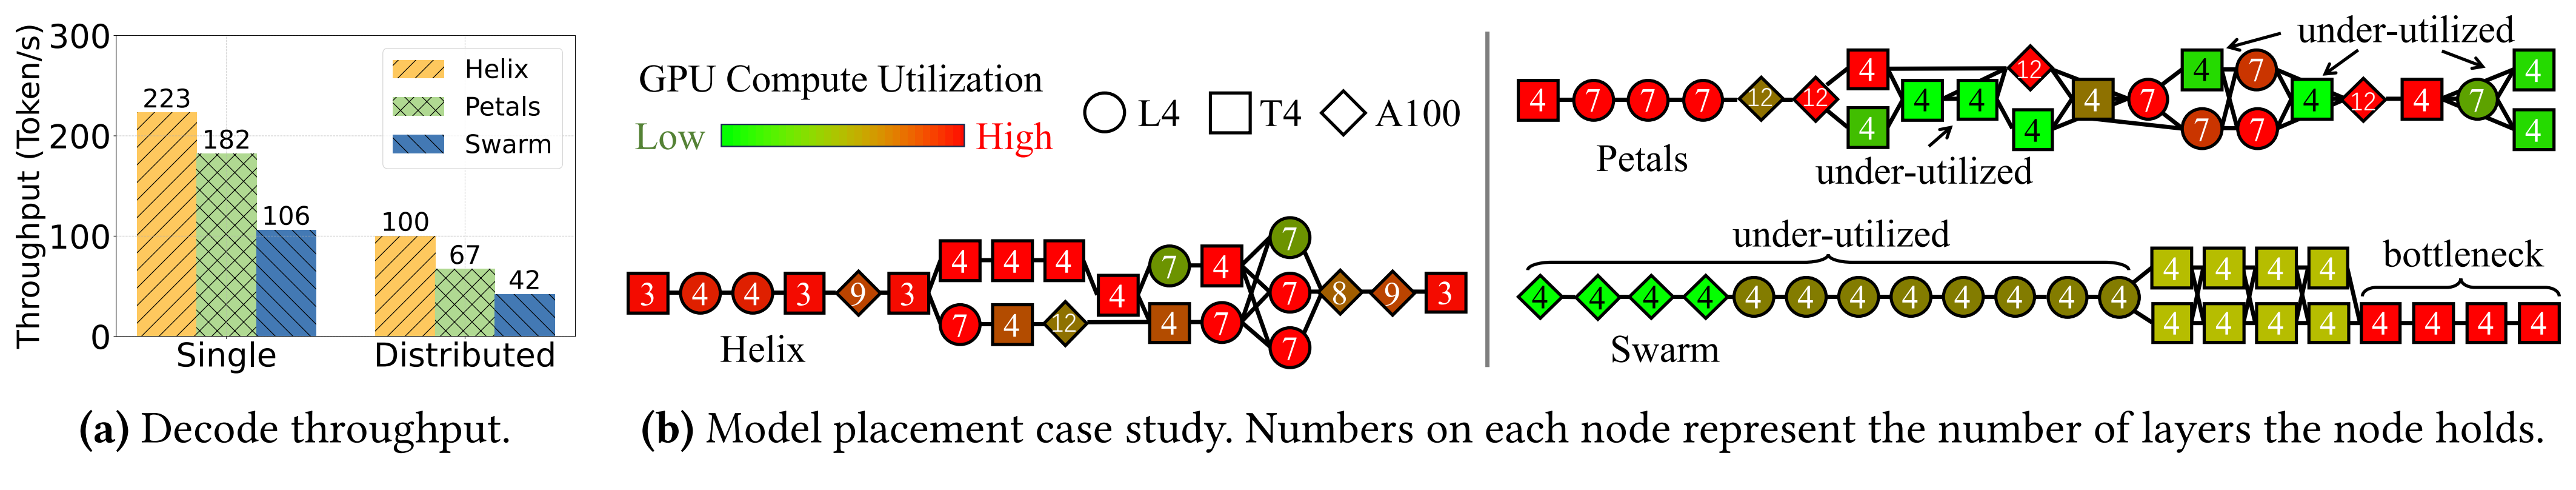
\includegraphics[width=\linewidth,trim=1000bp 160bp 0 0,clip]{Helix/Without-Caption/Helix_Figure_09_Model_Placement_Comparison.png}\par}
\medskip
{\small Node numbers are layer counts; color shows GPU compute utilization.\par\medskip
Swarm's tail bottleneck leaves faster GPUs under-used. Helix keeps almost every node busy.\par}
\src{Sec.~6.6, Fig.~9(b), enlarged crop. Full figure on Main 14.}
\back[\nav{B29}{Detailed Ratios}]{M13}
\end{frame}

\begin{frame}[c,label=B29]{Model Placement Deep Dive}
\vspace*{\fill}
\vspace{.02cm}

  {\centering\hint{Fig.~9. Offline LLaMA 70B. Every method uses Helix's scheduler. Integers in (b) are layer counts.}\par}
  \vspace{.03cm}
  \begin{itemize}\small
    \setlength{\itemsep}{.04cm}
    \item Vs.\ Petals / Swarm: \(1.23\times\) / \(2.10\times\) on the single cluster, and \(1.49\times\) / \(2.38\times\) on the geo-distributed simulator.
    \item Single-cluster case: Swarm's tail is four T4s with four layers each, so A100 and L4 stay under-used.
    \item Petals leaves eight T4s and one L4 under-used. Helix's plan keeps almost every node busy.
  \end{itemize}

  \src{Sec.~6.6, Fig.~9. PDF p.~11. Petals is not an end-to-end baseline.}
\back[\nav{BASELINES}{Main 10} \nav{FIG9}{Graph Detail}]{M13}
\end{frame}

\begin{frame}[c,label=FIG10]{Figure 10: Scheduling Graph Detail}
\vspace*{\fill}
\meta{Geo-distributed case study. Same Helix placement; scheduling can congest slow links.}
{\centering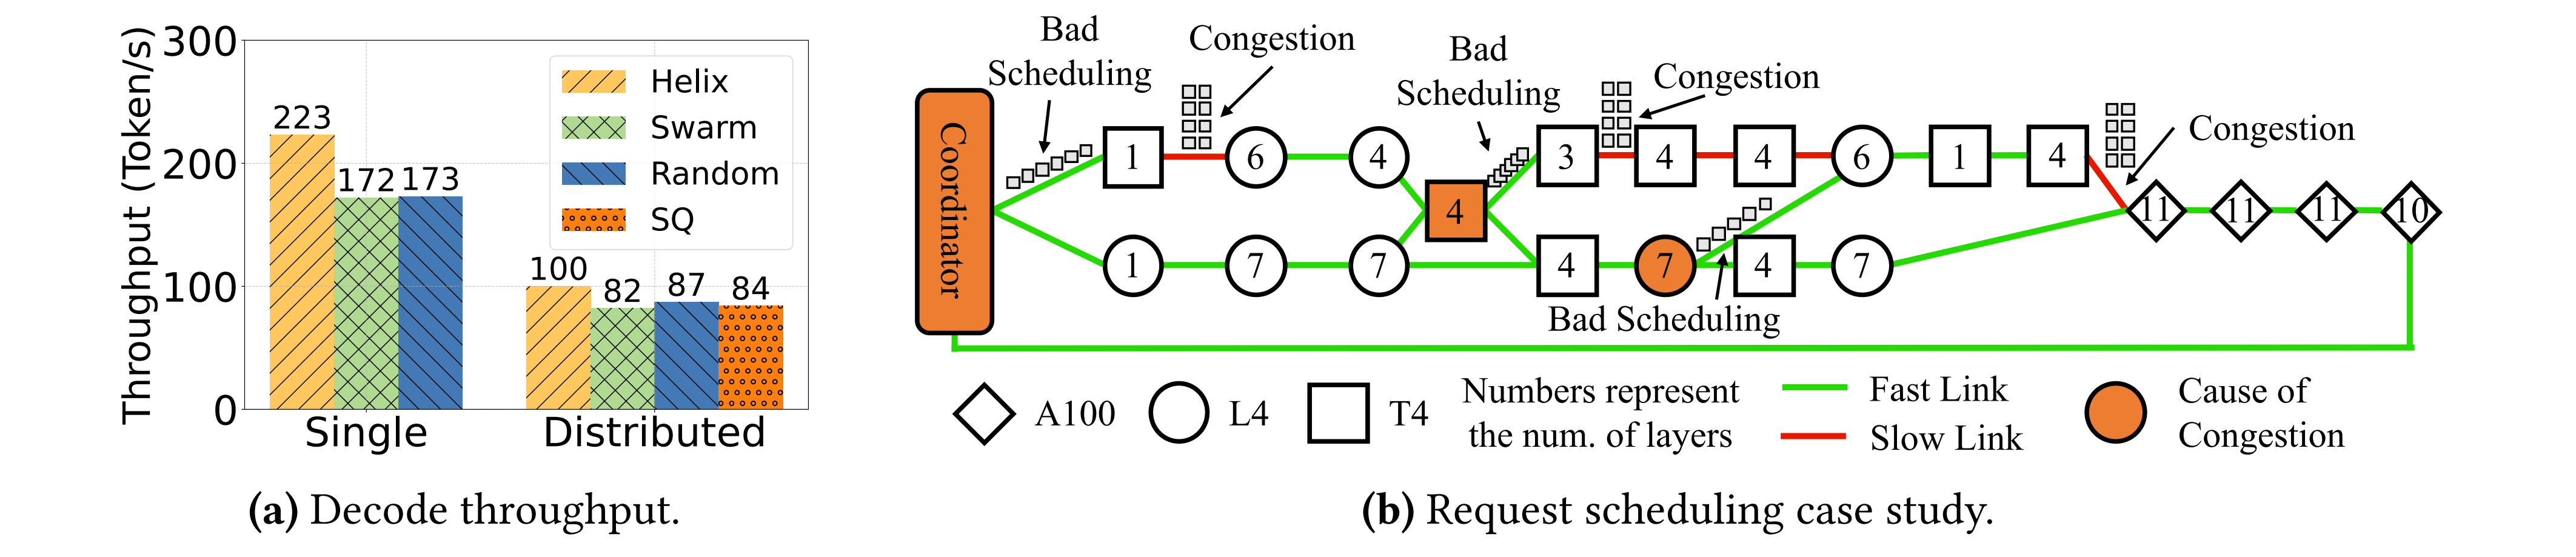
\includegraphics[width=\linewidth,trim=1400bp 170bp 0 0,clip]{Helix/Without-Caption/Helix_Figure_10_Request_Scheduling_Comparison.png}\par}
\medskip
{\small Orange nodes mark scheduling decisions that cause congestion.\par\medskip
Prompt traffic waits 5--16 s on three slow links; one queue is caused three hops upstream.\par}
\src{Sec.~6.7, Fig.~10(b), enlarged crop. Full figure on Main 15.}
\back[\nav{B30}{Detailed Ratios}]{M14}
\end{frame}

\begin{frame}[c,label=B30]{Request Scheduling Deep Dive}
\vspace*{\fill}
\vspace{.02cm}

  {\centering\hint{Fig.~10. Offline LLaMA 70B. Every method uses Helix's placement. (b) is the geo-distributed case study.}\par}
  \vspace{.03cm}
  \begin{itemize}\small
    \setlength{\itemsep}{.04cm}
    \item Vs.\ Swarm / random: \(+30\%\) / \(+29\%\) on the single cluster, and \(+22\%\) / \(+15\%\) on the geo-distributed clusters.
    \item Vs.\ shortest queue, geo-distributed only: \(+19\%\) decode throughput.
    \item In (b), prompt traffic waits 5--16 s on three slow links. One of those queues is caused by a scheduler three hops away.
  \end{itemize}

  \src{Sec.~6.7, Fig.~10. PDF p.~12.}
\back[\nav{FIG10}{Graph Detail}]{M14}
\end{frame}

\begin{frame}[c,label=B31]{MILP Optimization Ablation}
\vspace*{\fill}
\figureplaceholder{Helix/Without-Caption/Helix_Figure_11_MILP_Optimization_Ablation.png}{2.8cm}{Figure 11}
\smallskip
{\small\centering
\begin{tabular}{lcc}\toprule
Offline 70B & 24-node geo & 42-node heterogeneous\\\midrule
Variables / constraints, pruned & 876 / 1122 & 2144 / 2772\\
Variables / constraints, unpruned & 1376 / 1848 & 4004 / 5502\\
Links removed / problem-size reduction & 50\% / 36\% & 72\% / 46\%\\
Throughput gain with pruning & 16\% & 2\%\\
Warm-start time saved (bars) & 30\% & 7.2\%\\\bottomrule
\end{tabular}\par}
\smallskip
{\small Degree-12 pruning eases the timed search; it does not prove deleted links useless. Warm start finds the same placement, with $1.43\times$ / $1.08\times$ solver speedup.\par}
\src{Sec.~6.8, Fig.~11, Table 8. Text says 43\% / 8\% less time; bars imply 30\% / 7.2\%.}
\back[\nav{B17}{Solver Settings}\nav{B32}{Solver Quality}]{M06}
\end{frame}

\begin{frame}[c,label=B32]{Solver Time and Solution Quality}
\vspace*{\fill}
\vspace{.02cm}
  \begin{columns}[c,onlytextwidth]
    \begin{column}{.48\textwidth}
      {\small\begin{itemize}\setlength{\itemsep}{.16cm}
        \item Instance: LLaMA 30B on 4 L4s and 6 T4s. This is smaller than the 24- and 42-node runs.
        \item The best feasible placement reaches the optimum in under 5 minutes.
        \item Certifying that optimum takes more than an hour of branch-and-bound.
        \item The red dotted line is that cluster's optimal throughput. The upper bound tightens as cuts are added.
      \end{itemize}}
      \par\smallskip{\small Early stop is reasonable here. Fig.~12 does not certify the 42-node plan.}\par
    \end{column}
    \begin{column}{.50\textwidth}
      \figureplaceholder{Helix/Without-Caption/Helix_Figure_12_MILP_Solution_Quality.png}{4.85cm}{Figure 12}
    \end{column}
  \end{columns}
  \src{Sec.~6.9, Fig.~12. PDF p.~13.}
\back{M06}
\end{frame}

\section{E: Discussion}
\begin{frame}[c,label=B33]{Limitations and Threats to Validity}
\vspace*{\fill}
\vspace{.08cm}
  \begin{itemize}\small
    \setlength{\itemsep}{.16cm}
    \item Placement is computed once. A workload shift does not trigger a new MILP in the described runtime.
    \item Geo-distributed and 42-node numbers are simulated. The \(<5\%\) error is a single-cluster prototype check.
    \item The KV mask uses average output length. The paper does not specify the high-water mark.
    \item Pruning and the 10-minute stall rule mean a deployed plan need not be a proven optimum.
    \item Decode latency can rise when Helix actually uses the slow GPUs that SP leaves idle.
    \item Evidence is FP16 LLaMA-1 30B and LLaMA-2 70B on one pruned Azure trace. The conclusion's ``guaranteed optimal'' is the MILP's claim, not every timed run.
  \end{itemize}

  \src{Sec.~4.5, Sec.~6, and Sec.~8. The last bullet contrasts the conclusion with Sec.~6.2 and Sec.~6.9.}
\back{M15}
\end{frame}

\begin{frame}[c,label=FUTURE]{Research Directions and Applicability}
\vspace*{\fill}
\point{Static placement}{How much throughput gain justifies weight movement and KV migration?}
\point{KV estimation}{Could output-length uncertainty guide admission without wasting VRAM?}
\point{Latency trade-offs}{Can SLO-constrained goodput replace pure throughput while retaining a tractable model?}
\point{Workload sensitivity}{Re-test different prompt/decode mixes, burstiness, bandwidth variation, and failures.}
\point{Evidence gap}{Validate geographically distributed execution and larger heterogeneous clusters on hardware.}
\src{Interpretation / research extensions motivated by Helix, Secs.~4.5, 5.2, 6.2--6.9. Not implemented by the paper.}\back{M15}

\end{frame}

\end{document}
